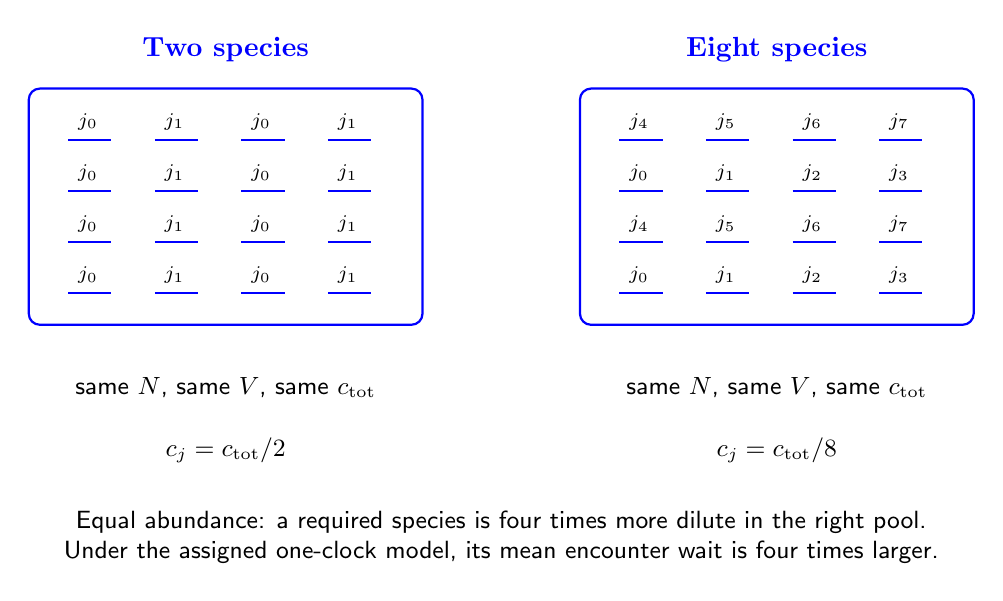
\begin{tikzpicture}[x=1cm,y=1cm,font=\small\sffamily]
\foreach \shift/\title in {0/{Two species},7/{Eight species}}{
\begin{scope}[xshift=\shift cm]
\draw[Blue,thick,rounded corners] (0,0) rectangle (5,3);
\node[Blue,font=\bfseries] at (2.5,3.5) {\title};
\foreach \i in {0,...,15}{
\pgfmathtruncatemacro{\col}{mod(\i,4)}
\pgfmathtruncatemacro{\row}{int(\i/4)}
\pgfmathtruncatemacro{\kind}{mod(\i,2)}
\ifnum\shift>0 \pgfmathtruncatemacro{\kind}{mod(\i,8)}\fi
\draw[Blue,thick] (.5+\col*1.1,.4+\row*.65)--++(.55,0);
\node[above,font=\scriptsize] at (.75+\col*1.1,.4+\row*.65) {$j_{\kind}$};}
\node[align=center] at (2.5,-.8) {same $N$, same $V$, same $c_{\rm tot}$};
\ifnum\shift=0 \node at (2.5,-1.6) {$c_j=c_{\rm tot}/2$};\else
\node at (2.5,-1.6) {$c_j=c_{\rm tot}/8$};\fi
\end{scope}}
\node[align=center] at (6,-2.7) {Equal abundance: a required species is four times more dilute in the right pool.\\
Under the assigned one-clock model, its mean encounter wait is four times larger.};
\end{tikzpicture}
